\documentclass[../Head/Main.tex]{subfiles}
\begin{document}
\section{Final Acceptance Test}
\label{sec:final_acceptance_test}

In this section an evaluation and explanation of the final acceptance test are made:

\textbf{Weather Conditions:}\\
The day of the final acceptance test, the weather was cold, however the sun was still shining, there was no rain and a light breeze. These conditions are very nice for testing, since it was not too shiny/bright or windy.

\subsection{Test Setup}
\label{subsec:test_setup}
The test was performed as stated in \autoref{subsec:req_UAS}. Two sets of GPS coordinates were manually captured using the GPS module on the drone. This was used as waypoints that the drone should follow along the fence. The path was visualized using QGroundControl's flight log import tool, see \autoref{fig:drone_traj_and_pov} along with a image of the drone.

\begin{figure}[H]
    \centering
    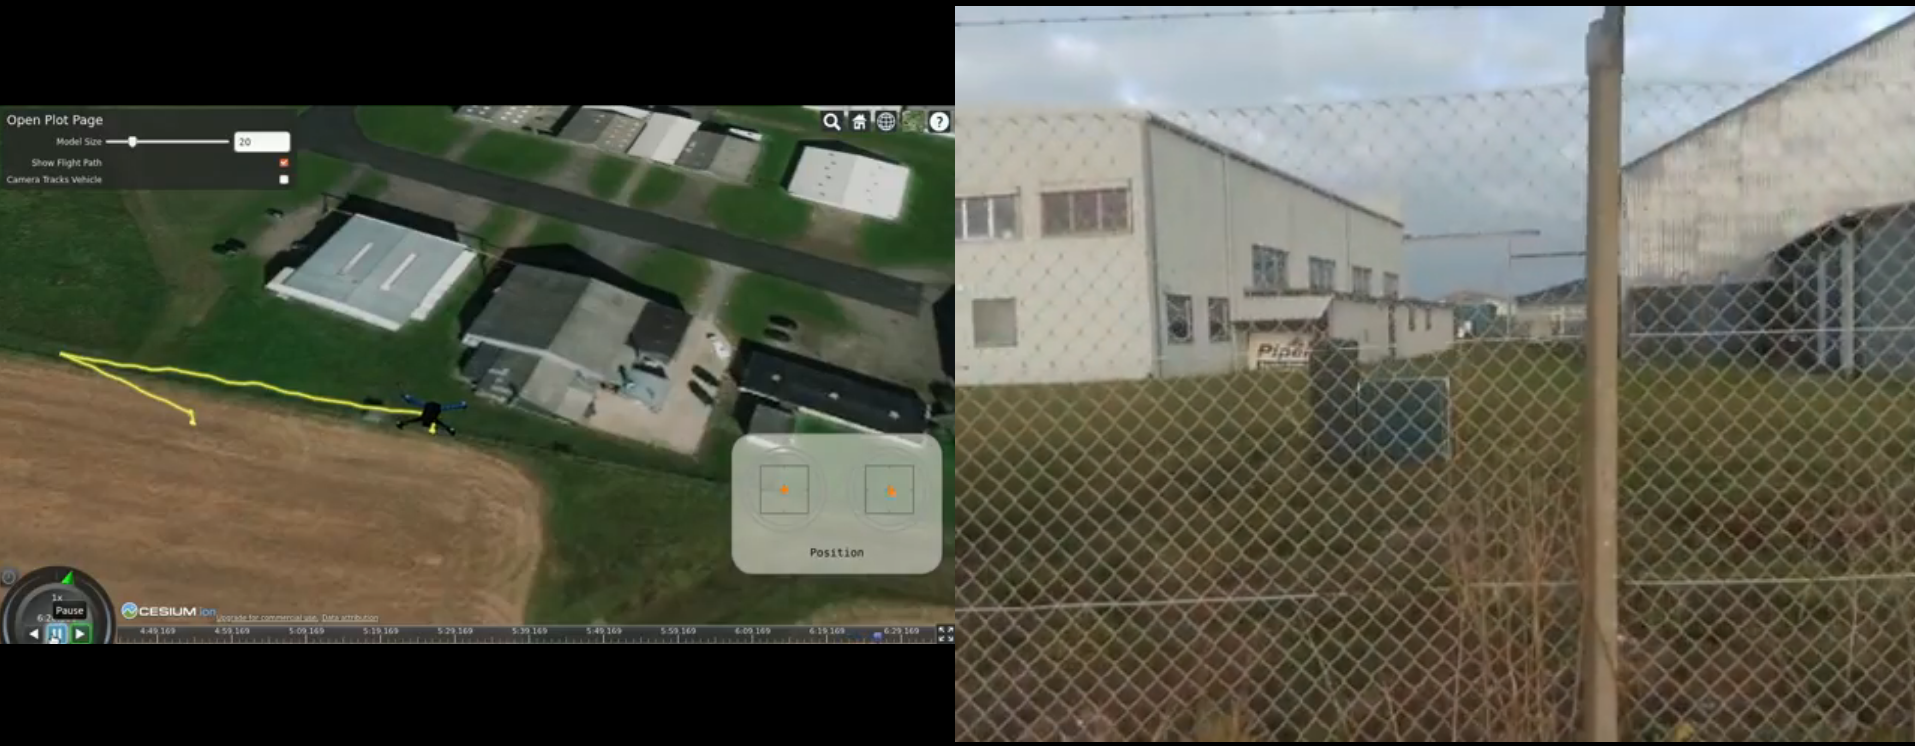
\includegraphics[width = 1.0\textwidth]{../Figures/pov_and_path.png}
    \caption{Drone trajectory and point of view}
    \label{fig:drone_traj_and_pov}
\end{figure}

It can be seen that it follows the route as intended. However, by analysing the final acceptance test video, which can be found on GitHub \cite{EiTGroup175}, it was noticed that the drones flight height differs a lot. Multiple runs using the same mission was performed and the height changes from test to test, and it was estimated to be due to the fluctuation in GPS data. Therefore it could have been beneficial to utilise another sensor to maintain height to the ground, while also using another sensor to maintain a certain distance to the fence, to make sure that the whole fence is visible by the camera. It can also be seen in the Point of view (POV) video that the drone's distance to the fence fluctuate, and sometimes the bottom part of the fence is not visible, which is not desirable.\\
The mission was started by our pilot using the controller, the same applies for starting and ending the recording of data. Each image is saved with a GPS, time, and date stamp as a package for further use when alerting the end-user about the position and time of breach location. 

\clearpage
\subsection{Analysis of test}
\label{subsec:test_result}
The mask-rcnn will be used in this section for breach detection which is explained in \autoref{subsec:deep_learning_cnn}. The video used in this analysis has been taken by the drone and split up into images which is going to be used in the mask-rcnn algorithm for breach prediction. This can be seen in \autoref{fig:real_life_test}.\\  
The drone was able to follow the desired path. However, the fluctuation in height and distance to the fence is not solved yet and is a troublesome problem that needs to be dealt with for this solution to be applicable. The pilot was able to start the mission and recording as intended. The camera was for the most time able to capture the whole fence but sometimes it flew a bit to high, which is unwanted.\\
As seen in \autoref{fig:real_life_test}, the drone detects the placed custom breaches (cardboard) located on the fence. However, also wrong detections are predicted. Some errors are seen because the algorithm falsely detects some grass in front of the fence in \autoref{fig:false_grass_1} and \autoref{fig:false_grass2}. The fence needs to be properly cleared of any obstructions in order to locate the breaches correctly. In \autoref{fig:false_window1}, \autoref{fig:false_windows2} and \autoref{fig:false_windows_3} windows are predicted to belonging to a breach class. This is due to the fact that the buildings matches the colour of the fence quite well and hence yields wrong detections. A way to accommodate for this could be to point the camera on the drone downwards to avoid seeing the buildings in the background and hence reduce the risk of wrong detections.  

\begin{figure}[H]
    \centering
    \begin{subfigure}{.23\textwidth}
        \centering
        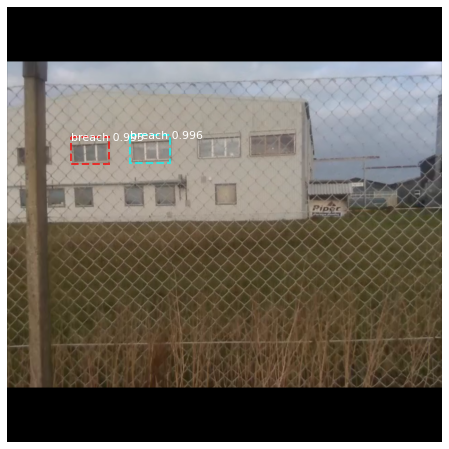
\includegraphics[width=\textwidth]{../Figures/rcnn_results/found_breaches/real_life_test/6.png}
        \caption{}
        \label{fig:false_window1}
    \end{subfigure}
    \hfill
    \begin{subfigure}{.23\textwidth}
        \centering
        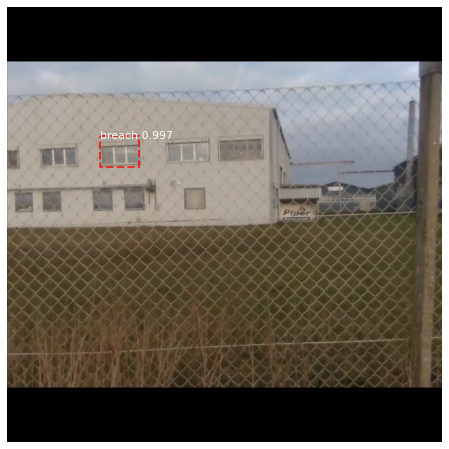
\includegraphics[width=\textwidth]{../Figures/rcnn_results/found_breaches/real_life_test/8.png}
        \caption{}
        \label{fig:false_windows2}
    \end{subfigure}
    \hfill
    \begin{subfigure}{.23\textwidth}
        \centering
        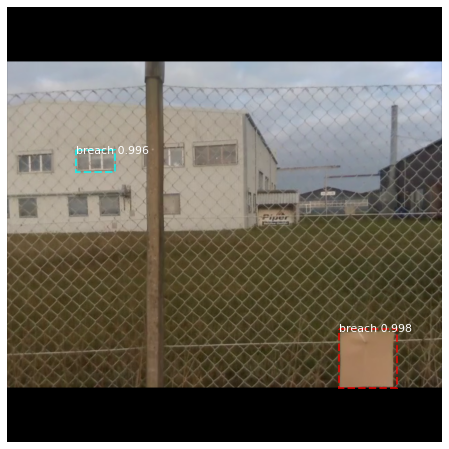
\includegraphics[width=\textwidth]{../Figures/rcnn_results/found_breaches/real_life_test/11.png}
        \caption{}
         \label{fig:false_windows_3}
    \end{subfigure}
    \hfill
    \begin{subfigure}{.23\textwidth}
        \centering
        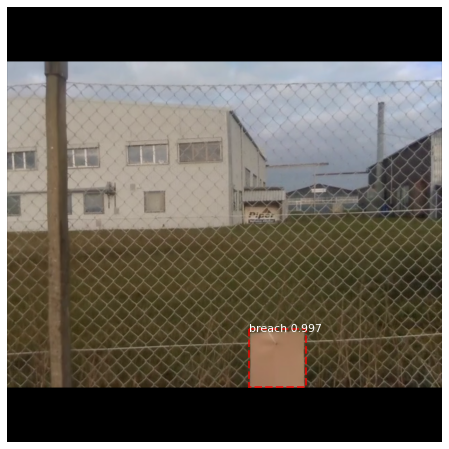
\includegraphics[width=\textwidth]{../Figures/rcnn_results/found_breaches/real_life_test/12.png}
        \caption{}
    \end{subfigure}
    \hfill
    \begin{subfigure}{.23\textwidth}
        \centering
        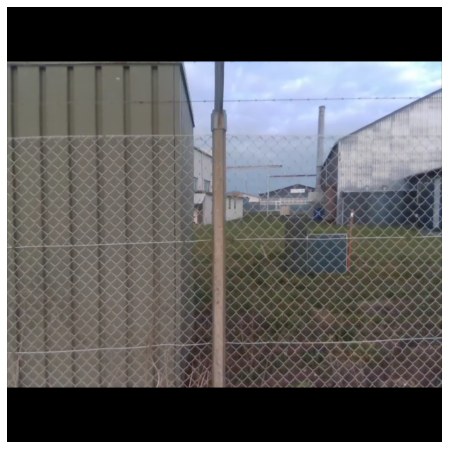
\includegraphics[width=\textwidth]{../Figures/rcnn_results/found_breaches/real_life_test/22.png}
        \caption{}
    \end{subfigure}
    \hfill
    \begin{subfigure}{.23\textwidth}
        \centering
        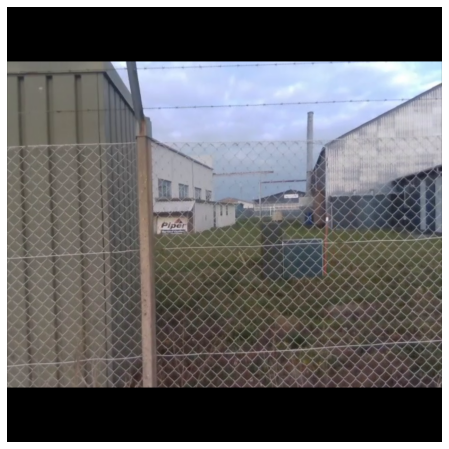
\includegraphics[width=\textwidth]{../Figures/rcnn_results/found_breaches/real_life_test/23.png}
        \caption{}
    \end{subfigure}
    \hfill
    \begin{subfigure}{.23\textwidth}
        \centering
        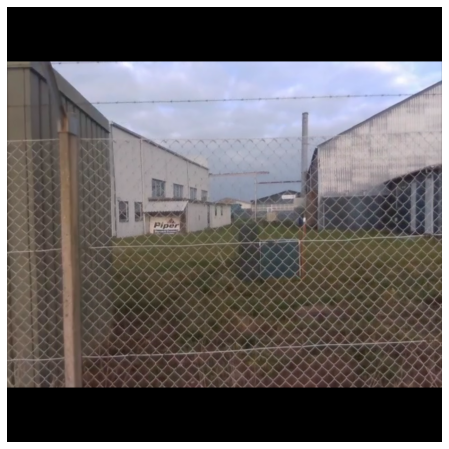
\includegraphics[width=\textwidth]{../Figures/rcnn_results/found_breaches/real_life_test/24.png}
        \caption{}
    \end{subfigure}
    \hfill
    \begin{subfigure}{.23\textwidth}
        \centering
        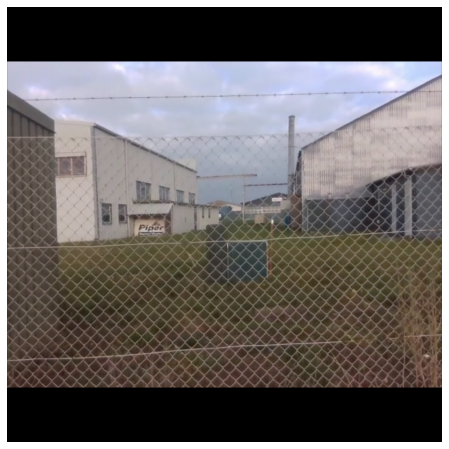
\includegraphics[width=\textwidth]{../Figures/rcnn_results/found_breaches/real_life_test/25.png}
        \caption{}
    \end{subfigure}
    \hfill
    \begin{subfigure}{.23\textwidth}
        \centering
        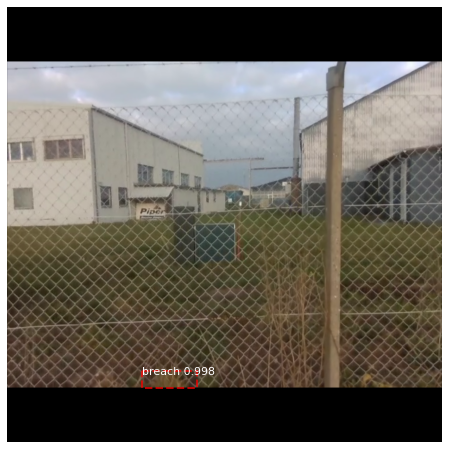
\includegraphics[width=\textwidth]{../Figures/rcnn_results/found_breaches/real_life_test/27.png}
        \caption{}
        \label{fig:false_grass_1}
    \end{subfigure}
    \hfill
    \begin{subfigure}{.23\textwidth}
        \centering
        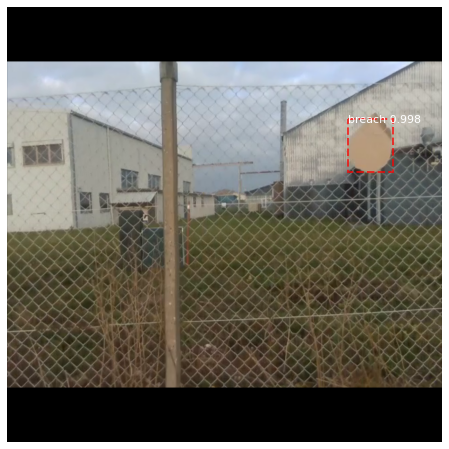
\includegraphics[width=\textwidth]{../Figures/rcnn_results/found_breaches/real_life_test/29.png}
        \caption{}
    \end{subfigure}
    \hfill
    \begin{subfigure}{.23\textwidth}
        \centering
        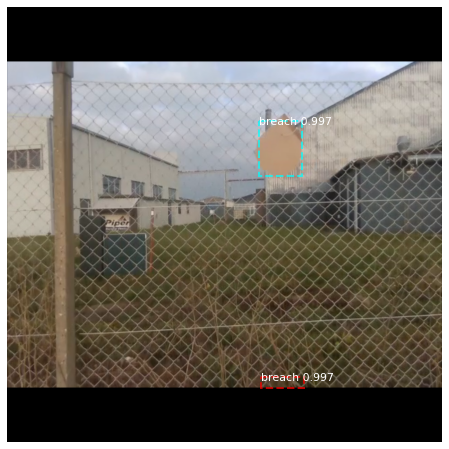
\includegraphics[width=\textwidth]{../Figures/rcnn_results/found_breaches/real_life_test/30.png}
        \caption{}
        \label{fig:false_grass2}
    \end{subfigure}
    \hfill
    \begin{subfigure}{.23\textwidth}
        \centering
        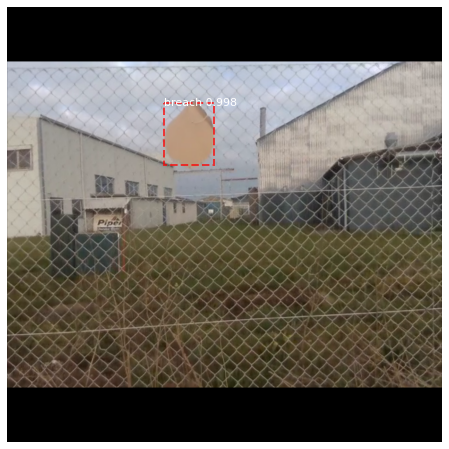
\includegraphics[width=\textwidth]{../Figures/rcnn_results/found_breaches/real_life_test/31.png}
        \caption{}
    \end{subfigure}
    \caption{Illustration of some of the images where the mask-rcnn correctly detects the cardboard placed on the fence. However, also minor false detections can be seen}
     \label{fig:real_life_test}
\end{figure}

Overall the test went quite well, but with minor difficulties that needs to be addressed going forward.  

\end{document}